% !TEX encoding = UTF-8 Unicode 
% !TEX root = praca.tex
\chapter{Tytuł rozdziału I}\label{chapter:ch1}

W książce \cite{docker_compose_reference} \dots

\section{Rysunki}

\begin{figure}
	\centering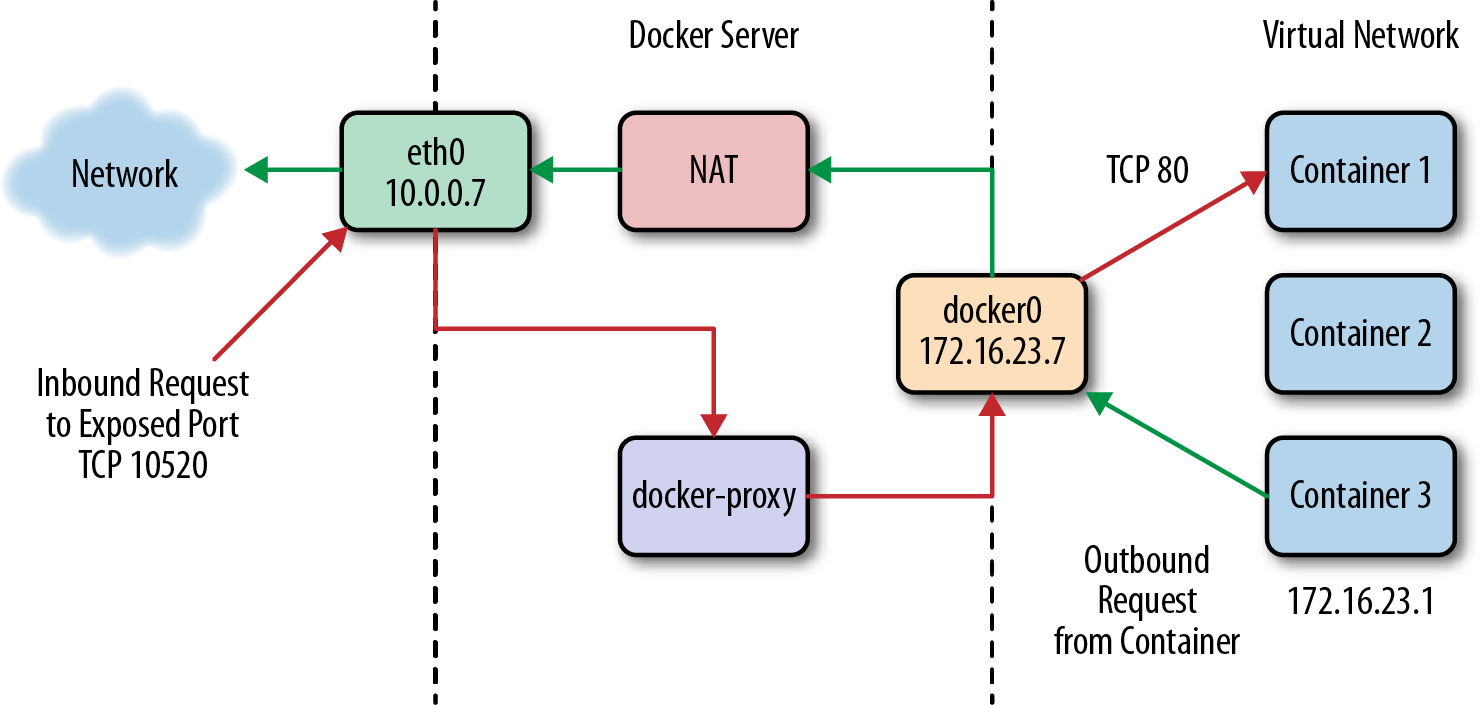
\includegraphics[width=.6\textwidth]{chapters/chapter1/imgs/swarm-network.png}
	\caption{Sieć dokera \cite{docker_compose_reference}}  \label{rys:network}
\end{figure}

Na rysunku \ref{rys:network} \dots


\subsection{Dwa rysunki obok siebie}

\begin{figure}[ht]
	\centering
	\begin{minipage}[b]{0.45\textwidth}
		\centering
\includegraphics[width=0.9\textwidth]{chapters/chapter1/imgs/kotek.pdf} % left figure
		\caption{Lewy rysunek}\label{fig:lewy}
	\end{minipage}
	\begin{minipage}[b]{0.45\textwidth}
		\centering
		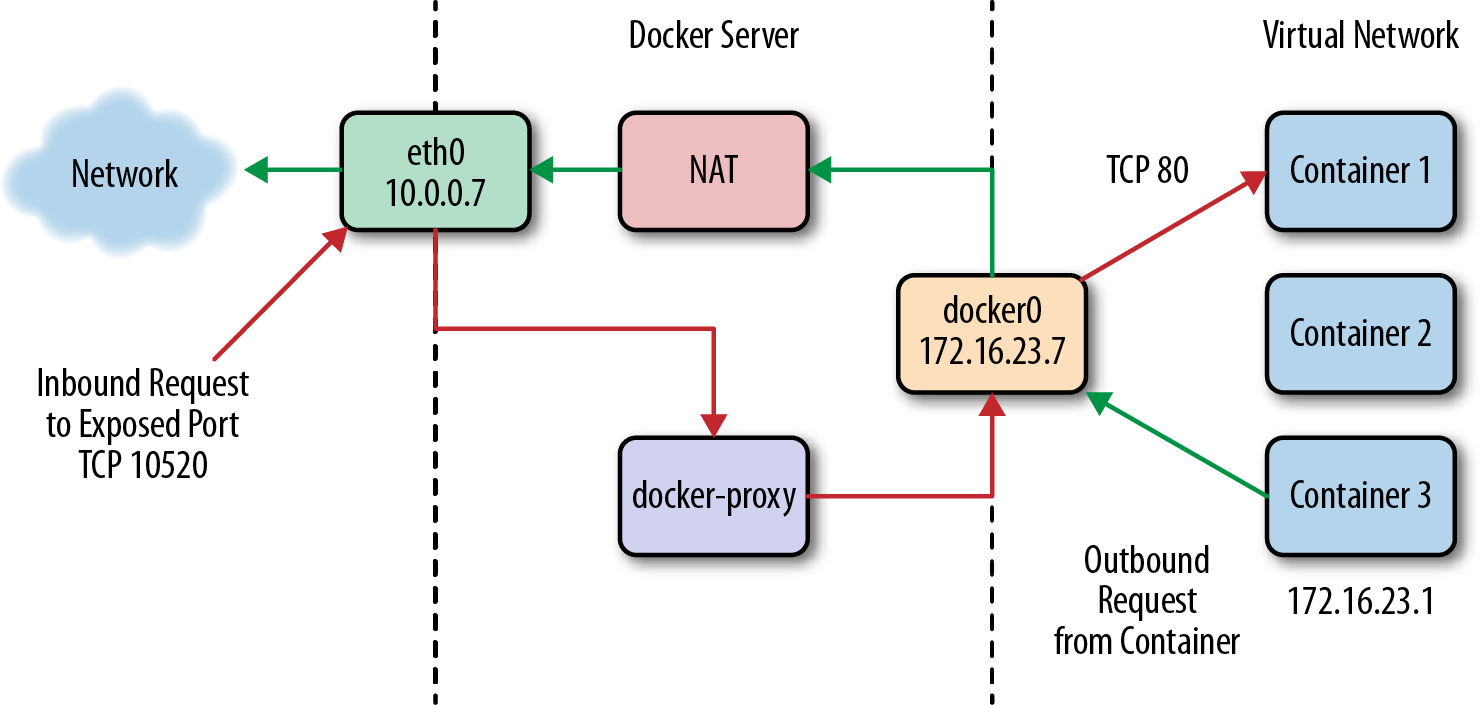
\includegraphics[width=0.9\textwidth]{chapters/chapter1/imgs/swarm-network.png} % right figure
		\caption{Prawy rysunek}\label{fig:prawy}
	\end{minipage}
\end{figure}

Na rysunkach \ref{fig:lewy} i \ref{fig:prawy} \dots


\section{Tabele}

W tabeli \ref{table:table1} \dots

\begin{table}
	\centering\caption{Tytuł tabeli (patrz dodatek~\ref{app1}) \label{table:table1}}
	\begin{tabular}{|l|l|l|}% table alignment -> l c r - left, center, right
		\hline
		Pierwszy & Drugi & Trzeci \\
		\hline
		Pierwszy & Drugi & Trzeci \\
		\hline
	\end{tabular}
\end{table}

\subsection{Równania}

\begin{equation}
	\sum_{i=1}^{\infty}a_i
	\label{eq:myEquation}
\end{equation}

W równaniu \ref{eq:myEquation} \dots

\section{Listingi}

Na listingu \ref{listing:myListing} \dots

% replace {c} with the appropriate language
\begin{listing}
	\begin{minted}{c}  
int main()
{
   int a=2*3;
   printf("**Ala ma kota\n**");
   while(!I2C_CheckEvent(I2C1, I2C_EVENT_MASTER_MODE_SELECT)); /* EV5 */
   return 0;
}
\end{minted}
	\caption{Język C} \label{listing:myListing}
\end{listing}

